\documentclass[12pt]{article}
\usepackage{anyfontsize}
\usepackage[a4paper, margin=2cm]{geometry}
\usepackage{polski}
\usepackage{tabto}
\usepackage{enumitem}
\usepackage{amsmath}
\usepackage{amssymb}
\usepackage{multirow}
\usepackage{multicol}
\usepackage{setspace}
\usepackage{pdfpages}
\usepackage{subcaption}



\usepackage{tabularx}
\newcolumntype{C}{>{\centering\arraybackslash}X}
\newcolumntype{L}{>{\raggedleft\arraybackslash}X}
\newcolumntype{R}{>{\raggedright\arraybackslash}X}
\newcommand{\centerY}[2]{\multirow{#1}{*}{#2}}

\usepackage{wrapfig}

\usepackage{hyperref}
\hypersetup{
    colorlinks = true,
    urlcolor=blue,
    linkcolor= black
}

\usepackage{chngcntr}
\counterwithin{figure}{section}
\counterwithin{table}{section}
\numberwithin{equation}{section}

\usepackage{graphicx}
\graphicspath{{./Img/}}

\usepackage{csvsimple}
\usepackage{pgfplots}
\usepackage{pgfplotstable}
\pgfplotsset{compat= newest}


\usepackage{titlesec}
\titlelabel{\thetitle.\quad}
% \AddToHook{cmd/section/before}{\clearpage}

\usepackage[european, american currents, americanvoltages, RPvoltages, cute inductor]{circuitikz}
\usepackage{tikz}
\usetikzlibrary{shapes.geometric}
\ctikzset{
    logic ports=ieee,
    logic ports/scale=0.75,
}

\usepgfplotslibrary{external}
\tikzexternalize[prefix=figs/]

\usepackage{csquotes}
\usepackage[sorting=none]{biblatex}
\bibliography{bibliography.bib}

\usepackage{listings}
\lstset{
literate=%
    {ą}{{\k{a}}}1
    {Ą}{{\k{A}}}1
    {ć}{{\'c}}1
    {Ć}{{\'{C}}}1
    {ę}{{\k{e}}}1
    {Ę}{{\k{E}}}1
    {ł}{{\l{}}}1
    {Ł}{{\L{}}}1
    {ń}{{\'n}}1
    {Ń}{{\'N}}1
    {ó}{{\'o}}1
    {Ó}{{\'O}}1
    {ś}{{\'s}}1
    {Ś}{{\'S}}1
    {ż}{{\.z}}1
    {Ż}{{\.Z}}1
    {ź}{{\'z}}1
    {Ź}{{\'Z}}1
}


\title{
    \includegraphics[width = 0.3\textwidth]{agh_logo.jpg}\\
    \textbf{Akademia Górniczo-Hutnicza w Krakowie}\\
    Wydział Informatyki, Elektroniki i  Telekomunikacji\\\vspace{2cm}
    \textbf{Raport z projektu}\\
    Title
}
\author{
    \begin{tabularx}{\textwidth}{l l}
    Autor: &Łukasz Przystupa\\
    Kierunek studiów: & Elektronika i Telekomunikacja\\
    \end{tabularx}
}
\date{\vspace{2cm}\today}

\usepackage{titling}
\renewcommand\maketitlehooka{\null\mbox{}\vfill}
\renewcommand\maketitlehookd{\vfill\null}

\usepackage{chngcntr}
\usepackage{etoolbox}
\newcounter{TaskCounter}[section]
\newcommand{\task}{
    \stepcounter{TaskCounter}
    \noindent\textbf{Zadanie \theTaskCounter:\\}
}



\begin{document}
    \begin{titlepage}
        \maketitle
        \thispagestyle{empty}
    \end{titlepage}

    \task
Narysuj i omów podstawowe układy pracy detektorów światła (IR, widzialnego, UV) opartych na fotodiodach:


\begin{figure}[!ht]
    \begin{subfigure}{0.35\textwidth}
        \centering
        \begin{circuitikz}
            \draw
                (0, 0) to[pD, i^= $I_{out}$] ++ (0, -2) to[R] ++ (0, -2) node[ground]{}
                (0, 0)  node[vcc]{Fotodioda}

                (4, -1) to[pD, invert, v= $V_{out}$] ++ (0, -2) node[ground]{}
                (4, -1)  node[vcc]{Panel}
            ;
        \end{circuitikz}
        \vspace{1.5cm}
    \end{subfigure}
% 
    \begin{subfigure}{0.6\textwidth}
        \centering
        \begin{tikzpicture}
            \begin{axis}[
                % width = 0.4\textwidth,
                grid = both,
                title = Charakterystyka prądowo napięciowa diody,
                xlabel = Napięcie,
                ylabel = Prad,
            ]
                \addplot[blue] table[x = Vd, y = Id, col sep = comma]{Measure/Diode.csv};
                \node at (-6, 0) [above right, align = center]{Zakres pracy\\ jako fotodioda};
                \node at (2, 0) [above, align = center]{Panel\\słoneczny};
            \end{axis}
        \end{tikzpicture}
    \end{subfigure}
\end{figure}

\begin{enumerate}
    \item Dioda w kierunku zaporowym - zachowuje się jako fotodioda.
    \item Dioda w kierunku przewodzenia to panel
\end{enumerate}

\task
Wymień i omów podstawowe parametry detektorów światła.

\begin{itemize}
    \item czułość
    \item długość fali
    \item prąd ciemny
    \item szum własny
    \item zakres pracy
    \item czas narastania
    \item wzmocnienie
    \item zależności temperaturowe
\end{itemize}


\task
Wymień i omów podstawowe parametry czujników temperatury
\begin{itemize}
    \item zakres pomiarowy - zakres temperatur jakie mogą być poprawnie mierzone za pomocą danego czujnika
    \item dokładność - różnica między temperaturą rzeczywistą a zmierzoną
    \item rozdzielczość - najmniejsza zmiana zauważona przez czujnik
    \item czas odpowiedzi - czas jaki czujnik potrzebuje aby ustalić wartość mierzoną
\end{itemize}

\newpage
\task
Narysuj i omów podstawowe układy pracy mierników temperatury opartych o termopary.

Termopara to czujnik temperatury zbudowany z dwóch różnych metali połączonych ze sobą w punkcie pomiarowym (punkt gorący).
Po drugiej stronie czujnika (zimne złącze) powstaje napięcie termoelektryczne proporcjonalne do różnicy temperatur.
\begin{figure}[!ht]
    \centering
    \begin{circuitikz}
        \draw
            (0, 0) node[draw, rectangle, minimum height = 2cm](termopara){Termopara}
            (6, 0) node[op amp](opAmp){}
            (opAmp.-) to[short, a=strona zimna] ++ (-3.7, 0)
            (opAmp.+) to[short, l=strona ciepła] ++ (-3.7, 0)

            (opAmp.out) to[adc,>] ++(2, 0) node[right, draw, rectangle, minimum width = 1cm, minimum height = 1cm]{$\mu C$}
        ;
    \end{circuitikz}
\end{figure}

\task
Wymień i omów podstawowe parametry czujników przyśpieszenia

\task
Wymień i omów podstawowe parametry czujników przesunięcia kątowego (żyroskopów)

\begin{itemize}
    \item zakres pomiarowy
    \item czułość
    \item rozdzielczość
    \item dokładność
    \item powtarzalność
    \item offset
    \item pasmo przenoszenia
    \item oś pomiaru
\end{itemize}

\task

\begin{wrapfigure}[4]{r}{0.5 \textwidth}
    \centering
    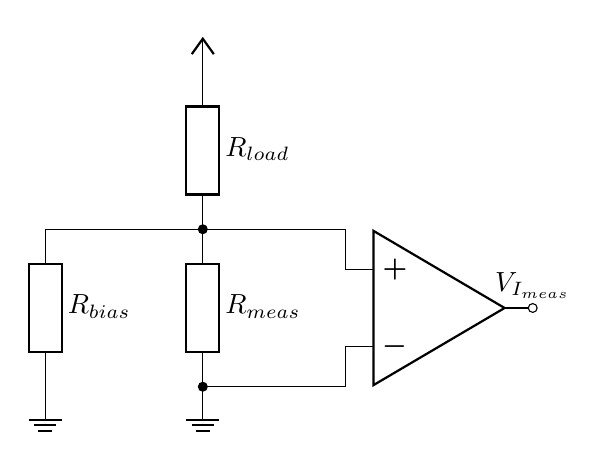
\begin{tikzpicture}
    \draw
        (0, 0) to[R = $R_{load}$] ++(0, -2)
            coordinate(A)
        to[R = $R_{meas}$, *-*] ++(0, -2)
            coordinate(B)

        (A) --++ (-2, 0) to[R = $R_{bias}$] ++ (0, -2) node[ground]{}
        (0, 0) node[vcc]{}
        (0, -4) node[ground]{}

        (3, -3) node[op amp, noinv input up](opAmp){}
        (A) -| (opAmp.+)
        (B) -| (opAmp.-)
        (opAmp.out) to[short, -o] ++ (0, 0) node[above]{$V_{I_{meas}}$}
    ;
    \end{tikzpicture}
\end{wrapfigure}

\noindent 
Narysuj i omów podstawowe układy pracy mierników prądu\\
Dla zakresu:
\begin{itemize}
    \item nA – uA - mA
    \item mA - 3A
    \item 10mA - 100A (500A)
\end{itemize}

\newpage
\task
Omów narażenia środowiskowe wpływające na działanie podzespołów i układów
elektronicznych
\begin{enumerate}
    \item Temperatura
    \begin{itemize}
        \item dryft napięcia półprzewodników
        \item zmiany pojemności i/lub rezystancji
        \item skrócenie żywotności elementu
    \end{itemize}
    \item Wilgotność
    \begin{itemize}
        \item prąd upływu
        \item korozja styków i wyprowadzeń
        \item zwarcia w obwodzie
    \end{itemize}
    \item Pył i brud
    \begin{itemize}
        \item problemy z chłodzeniem
    \end{itemize}
    \item Środki chemiczne
    \begin{itemize}
        \item przebicia, zwarcia,
        \item niszczenie obudów
    \end{itemize}
    \item Wibracje i wstrząsy
    \begin{itemize}
        \item pęknięcia, uszkodzenia struktur scalonych
        \item zwiększenie rezystancji połączeń (np. lutów)
    \end{itemize}
    \item Promieniowanie elektromagnetyczne:
    \begin{itemize}
        \item zaburzenia w pracy układów
        \item zmiany w pamięciach trwałych
        \item przegrzewanie się urządzeń
    \end{itemize}
    \item Wyładowania ESD
    \begin{itemize}
        \item zniszczenie elementów
        \item obniżenie żywotności
    \end{itemize}
    \item Ciśnienie pracy
    \begin{itemize}
        \item błędne odczyty
        \item obniżenie żywotności
    \end{itemize}
\end{enumerate}
\newpage

\task
\begin{figure}[!ht]
    \centering
    \begin{circuitikz}
    \draw
        (0, -1) node[draw, rectangle, minimum width = 2cm, minimum height = 2cm, align = center](A){$\mu C$}

        (3, 0) node[draw, rectangle, minimum width = 1cm, minimum height = 1cm, align = center](B){Generator\\impulsów}
        (7, 0) node[draw, rectangle, minimum width = 1cm, minimum height = 1cm, align = center](C){Nadajnik\\ultradźwiękowy}

        (12, -2) node[draw, rectangle, minimum width = 1cm, minimum height = 1cm, align = center](D){Odbiornik\\ultradźwiękowy}
        (9.5, -2) node[plain mono amp, scale = 0.5, rotate = 180](E){}
        (7, -2) node[draw, rectangle, minimum width = 1cm, minimum height = 1cm, align = center](F){Układ detekcji\\sygnałów}
        (3, -2) node[draw, rectangle, minimum width = 1cm, minimum height = 1cm, align = center](G){Układ pomiaru\\czasu}

        (B) -- (C)
        (D) -- (E.in)
        (E.out) -- (F) -- (G)
    ;
    \draw[-Stealth] (A) -- (B);
    \draw[-Stealth] (G) -- (A);
    \end{circuitikz}
\end{figure}
\end{document}
